\documentclass{standalone}
\usepackage{tikz}
\usetikzlibrary{patterns, positioning}


\begin{document}
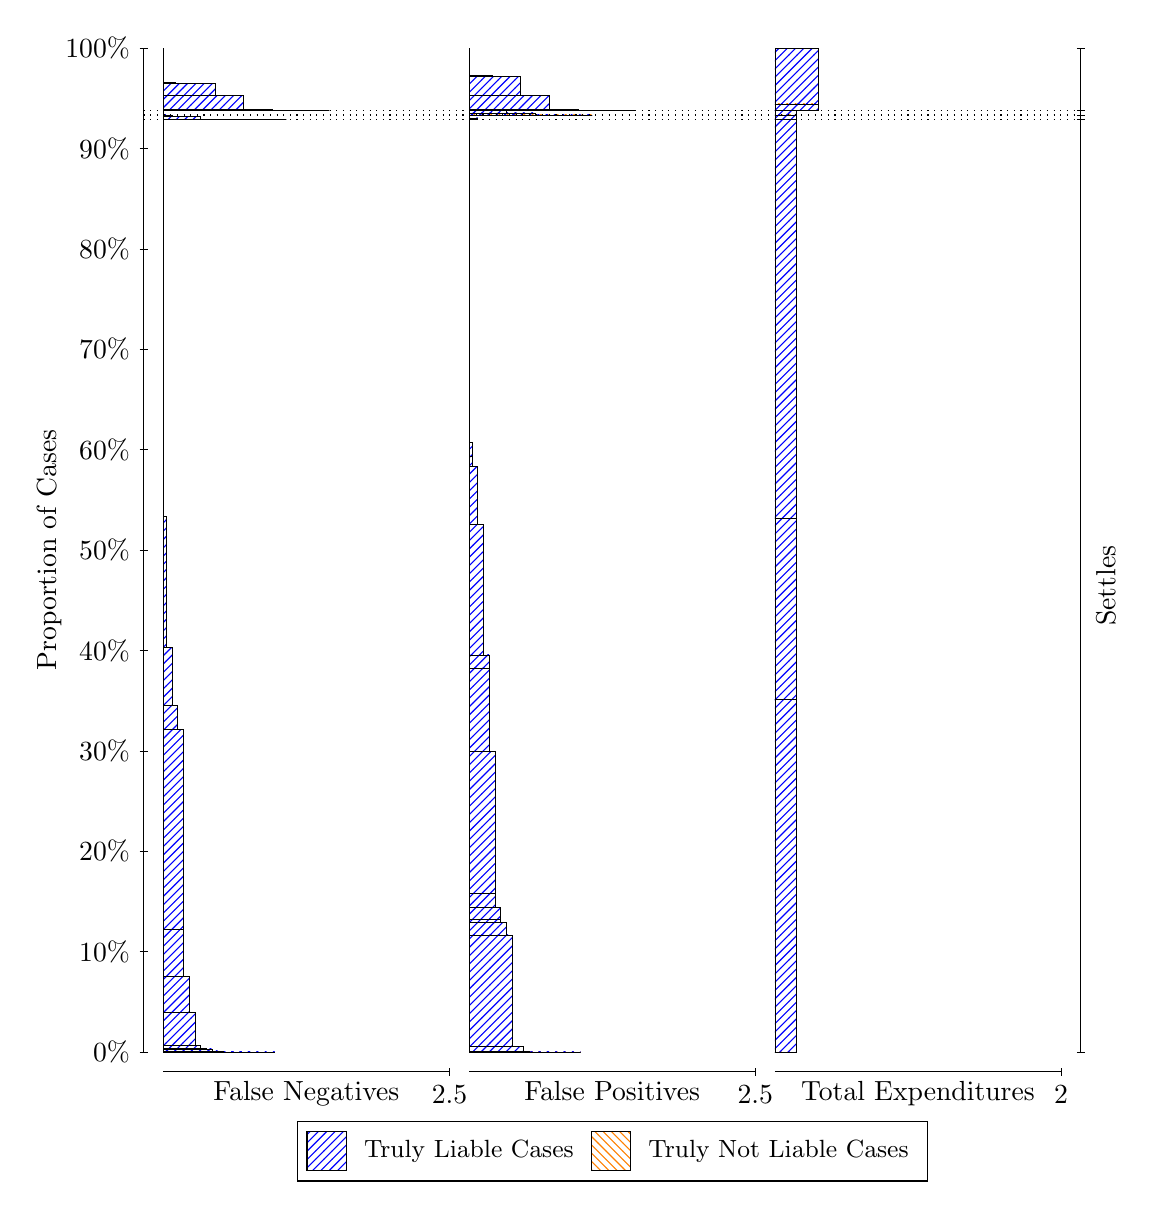
\begin{tikzpicture}
\draw[black, very thin] (1.5,1.75) -- (1.5,14.5);
\node[rotate=90, text=black, anchor=center] at (0.3, 8.125) {Proportion of Cases};
\draw[black, very thin] (1.45,1.75) -- (1.55,1.75);
\node[text=black, anchor=east] at (1.45, 1.75) {0\%};
\draw[black, very thin] (1.45,3.025) -- (1.55,3.025);
\node[text=black, anchor=east] at (1.45, 3.025) {10\%};
\draw[black, very thin] (1.45,4.3) -- (1.55,4.3);
\node[text=black, anchor=east] at (1.45, 4.3) {20\%};
\draw[black, very thin] (1.45,5.575) -- (1.55,5.575);
\node[text=black, anchor=east] at (1.45, 5.575) {30\%};
\draw[black, very thin] (1.45,6.85) -- (1.55,6.85);
\node[text=black, anchor=east] at (1.45, 6.85) {40\%};
\draw[black, very thin] (1.45,8.125) -- (1.55,8.125);
\node[text=black, anchor=east] at (1.45, 8.125) {50\%};
\draw[black, very thin] (1.45,9.4) -- (1.55,9.4);
\node[text=black, anchor=east] at (1.45, 9.4) {60\%};
\draw[black, very thin] (1.45,10.675) -- (1.55,10.675);
\node[text=black, anchor=east] at (1.45, 10.675) {70\%};
\draw[black, very thin] (1.45,11.95) -- (1.55,11.95);
\node[text=black, anchor=east] at (1.45, 11.95) {80\%};
\draw[black, very thin] (1.45,13.225) -- (1.55,13.225);
\node[text=black, anchor=east] at (1.45, 13.225) {90\%};
\draw[black, very thin] (1.45,14.5) -- (1.55,14.5);
\node[text=black, anchor=east] at (1.45, 14.5) {100\%};

\draw[black, very thin] (13.4,1.75) -- (13.4,14.5);
\draw[black, very thin] (13.35,1.75) -- (13.45,1.75);
\node[anchor=west] at (13.35, 1.75) {};
\draw[black, very thin] (13.35,13.593) -- (13.45,13.593);
\node[anchor=west] at (13.35, 13.593) {};
\draw[black, very thin] (13.35,13.65) -- (13.45,13.65);
\node[anchor=west] at (13.35, 13.65) {};
\draw[black, very thin] (13.35,13.705) -- (13.45,13.705);
\node[anchor=west] at (13.35, 13.705) {};
\draw[black, very thin] (13.35,14.5) -- (13.45,14.5);
\node[anchor=west] at (13.35, 14.5) {};

\draw[black, very thin, pattern color=blue, pattern=north east lines] (1.75,1.75) rectangle (3.167,1.75);
\draw[black, very thin, pattern color=blue, pattern=north east lines] (1.75,1.75) rectangle (3.0217,1.75);
\draw[black, very thin, pattern color=blue, pattern=north east lines] (1.75,1.75) rectangle (2.8763,1.75);
\draw[black, very thin, pattern color=blue, pattern=north east lines] (1.75,1.75) rectangle (2.8037,1.75);
\draw[black, very thin, pattern color=blue, pattern=north east lines] (1.75,1.75) rectangle (2.731,1.75);
\draw[black, very thin, pattern color=blue, pattern=north east lines] (1.75,1.75) rectangle (2.6583,1.75);
\draw[black, very thin, pattern color=blue, pattern=north east lines] (1.75,1.75) rectangle (2.5857,1.75);
\draw[black, very thin, pattern color=blue, pattern=north east lines] (1.75,1.75) rectangle (2.513,1.7555);
\draw[black, very thin, pattern color=blue, pattern=north east lines] (1.75,1.7555) rectangle (2.4403,1.7637);
\draw[black, very thin, pattern color=blue, pattern=north east lines] (1.75,1.7637) rectangle (2.3677,1.7893);
\draw[black, very thin, pattern color=blue, pattern=north east lines] (1.75,1.7893) rectangle (2.295,1.7968);
\draw[black, very thin, pattern color=blue, pattern=north east lines] (1.75,1.7968) rectangle (2.2223,1.831);
\draw[black, very thin, pattern color=blue, pattern=north east lines] (1.75,1.831) rectangle (2.1497,2.2521);
\draw[black, very thin, pattern color=blue, pattern=north east lines] (1.75,2.2521) rectangle (2.077,2.7107);
\draw[black, very thin, pattern color=blue, pattern=north east lines] (1.75,2.7107) rectangle (2.0043,3.3067);
\draw[black, very thin, pattern color=blue, pattern=north east lines] (1.75,3.3067) rectangle (2.0043,5.8484);
\draw[black, very thin, pattern color=blue, pattern=north east lines] (1.75,5.8484) rectangle (1.9317,6.1518);
\draw[black, very thin, pattern color=blue, pattern=north east lines] (1.75,6.1518) rectangle (1.859,6.8906);
\draw[black, very thin, pattern color=blue, pattern=north east lines] (1.75,6.8906) rectangle (1.7863,8.5506);
\draw[black, very thin, pattern color=orange, pattern=north west lines] (1.75,8.5506) rectangle (1.75,8.5506);
\draw[black, very thin, pattern color=blue, pattern=north east lines] (1.75,8.5506) rectangle (1.75,13.593);
\draw[black, very thin, pattern color=blue, pattern=north east lines] (1.75,13.593) rectangle (3.3123,13.593);
\draw[black, very thin, pattern color=blue, pattern=north east lines] (1.75,13.593) rectangle (2.949,13.593);
\draw[black, very thin, pattern color=blue, pattern=north east lines] (1.75,13.593) rectangle (2.5857,13.594);
\draw[black, very thin, pattern color=blue, pattern=north east lines] (1.75,13.594) rectangle (2.2223,13.629);
\draw[black, very thin, pattern color=blue, pattern=north east lines] (1.75,13.629) rectangle (1.859,13.65);
\draw[black, very thin, pattern color=orange, pattern=north west lines] (1.75,13.65) rectangle (1.75,13.65);
\draw[black, very thin, pattern color=blue, pattern=north east lines] (1.75,13.65) rectangle (1.859,13.65);
\draw[black, very thin, pattern color=orange, pattern=north west lines] (1.75,13.65) rectangle (1.75,13.65);
\draw[black, very thin, pattern color=blue, pattern=north east lines] (1.75,13.65) rectangle (1.75,13.705);
\draw[black, very thin, pattern color=blue, pattern=north east lines] (1.75,13.705) rectangle (3.8573,13.705);
\draw[black, very thin, pattern color=blue, pattern=north east lines] (1.75,13.705) rectangle (3.494,13.705);
\draw[black, very thin, pattern color=blue, pattern=north east lines] (1.75,13.705) rectangle (3.1307,13.721);
\draw[black, very thin, pattern color=blue, pattern=north east lines] (1.75,13.721) rectangle (2.7673,13.895);
\draw[black, very thin, pattern color=blue, pattern=north east lines] (1.75,13.895) rectangle (2.622,13.895);
\draw[black, very thin, pattern color=blue, pattern=north east lines] (1.75,13.895) rectangle (2.404,14.05);
\draw[black, very thin, pattern color=blue, pattern=north east lines] (1.75,14.05) rectangle (2.2587,14.05);
\draw[black, very thin, pattern color=blue, pattern=north east lines] (1.75,14.05) rectangle (2.0407,14.051);
\draw[black, very thin, pattern color=blue, pattern=north east lines] (1.75,14.051) rectangle (1.8953,14.061);
\draw[black, very thin, pattern color=orange, pattern=north west lines] (1.75,14.061) rectangle (1.75,14.061);
\draw[black, very thin, pattern color=blue, pattern=north east lines] (1.75,14.061) rectangle (1.75,14.5);
\draw[black, very thin, pattern color=orange, pattern=north west lines] (5.6333,1.75) rectangle (7.0503,1.75);
\draw[black, very thin, pattern color=blue, pattern=north east lines] (5.6333,1.75) rectangle (7.0503,1.75);
\draw[black, very thin, pattern color=orange, pattern=north west lines] (5.6333,1.75) rectangle (6.7597,1.75);
\draw[black, very thin, pattern color=blue, pattern=north east lines] (5.6333,1.75) rectangle (6.7597,1.75);
\draw[black, very thin, pattern color=blue, pattern=north east lines] (5.6333,1.75) rectangle (6.687,1.75);
\draw[black, very thin, pattern color=orange, pattern=north west lines] (5.6333,1.75) rectangle (6.6143,1.75);
\draw[black, very thin, pattern color=blue, pattern=north east lines] (5.6333,1.75) rectangle (6.6143,1.75);
\draw[black, very thin, pattern color=orange, pattern=north west lines] (5.6333,1.75) rectangle (6.469,1.75);
\draw[black, very thin, pattern color=blue, pattern=north east lines] (5.6333,1.75) rectangle (6.469,1.7523);
\draw[black, very thin, pattern color=blue, pattern=north east lines] (5.6333,1.7523) rectangle (6.3963,1.7527);
\draw[black, very thin, pattern color=orange, pattern=north west lines] (5.6333,1.7527) rectangle (6.3237,1.7527);
\draw[black, very thin, pattern color=blue, pattern=north east lines] (5.6333,1.7527) rectangle (6.3237,1.7551);
\draw[black, very thin, pattern color=blue, pattern=north east lines] (5.6333,1.7551) rectangle (6.3237,1.8192);
\draw[black, very thin, pattern color=blue, pattern=north east lines] (5.6333,1.8192) rectangle (6.251,1.821);
\draw[black, very thin, pattern color=orange, pattern=north west lines] (5.6333,1.821) rectangle (6.1783,1.821);
\draw[black, very thin, pattern color=blue, pattern=north east lines] (5.6333,1.821) rectangle (6.1783,3.2372);
\draw[black, very thin, pattern color=blue, pattern=north east lines] (5.6333,3.2372) rectangle (6.1057,3.3921);
\draw[black, very thin, pattern color=orange, pattern=north west lines] (5.6333,3.3921) rectangle (6.033,3.3921);
\draw[black, very thin, pattern color=blue, pattern=north east lines] (5.6333,3.3921) rectangle (6.033,3.4362);
\draw[black, very thin, pattern color=blue, pattern=north east lines] (5.6333,3.4362) rectangle (6.033,3.5826);
\draw[black, very thin, pattern color=blue, pattern=north east lines] (5.6333,3.5826) rectangle (5.9603,3.7612);
\draw[black, very thin, pattern color=blue, pattern=north east lines] (5.6333,3.7612) rectangle (5.9603,5.5653);
\draw[black, very thin, pattern color=orange, pattern=north west lines] (5.6333,5.5653) rectangle (5.8877,5.5653);
\draw[black, very thin, pattern color=blue, pattern=north east lines] (5.6333,5.5653) rectangle (5.8877,6.6274);
\draw[black, very thin, pattern color=blue, pattern=north east lines] (5.6333,6.6274) rectangle (5.8877,6.7925);
\draw[black, very thin, pattern color=blue, pattern=north east lines] (5.6333,6.7925) rectangle (5.815,8.4526);
\draw[black, very thin, pattern color=blue, pattern=north east lines] (5.6333,8.4526) rectangle (5.7423,9.1913);
\draw[black, very thin, pattern color=blue, pattern=north east lines] (5.6333,9.1913) rectangle (5.6697,9.3185);
\draw[black, very thin, pattern color=blue, pattern=north east lines] (5.6333,9.3185) rectangle (5.6697,9.4947);
\draw[black, very thin, pattern color=blue, pattern=north east lines] (5.6333,9.4947) rectangle (5.6333,13.593);
\draw[black, very thin, pattern color=orange, pattern=north west lines] (5.6333,13.593) rectangle (5.7423,13.593);
\draw[black, very thin, pattern color=blue, pattern=north east lines] (5.6333,13.593) rectangle (5.7423,13.614);
\draw[black, very thin, pattern color=blue, pattern=north east lines] (5.6333,13.614) rectangle (5.6333,13.65);
\draw[black, very thin, pattern color=orange, pattern=north west lines] (5.6333,13.65) rectangle (7.1957,13.65);
\draw[black, very thin, pattern color=blue, pattern=north east lines] (5.6333,13.65) rectangle (7.1957,13.65);
\draw[black, very thin, pattern color=blue, pattern=north east lines] (5.6333,13.65) rectangle (6.8323,13.65);
\draw[black, very thin, pattern color=blue, pattern=north east lines] (5.6333,13.65) rectangle (6.469,13.677);
\draw[black, very thin, pattern color=blue, pattern=north east lines] (5.6333,13.677) rectangle (6.1057,13.705);
\draw[black, very thin, pattern color=blue, pattern=north east lines] (5.6333,13.705) rectangle (5.7423,13.705);
\draw[black, very thin, pattern color=orange, pattern=north west lines] (5.6333,13.705) rectangle (7.7407,13.705);
\draw[black, very thin, pattern color=blue, pattern=north east lines] (5.6333,13.705) rectangle (7.7407,13.705);
\draw[black, very thin, pattern color=orange, pattern=north west lines] (5.6333,13.705) rectangle (7.3773,13.705);
\draw[black, very thin, pattern color=blue, pattern=north east lines] (5.6333,13.705) rectangle (7.3773,13.705);
\draw[black, very thin, pattern color=orange, pattern=north west lines] (5.6333,13.705) rectangle (7.014,13.705);
\draw[black, very thin, pattern color=blue, pattern=north east lines] (5.6333,13.705) rectangle (7.014,13.716);
\draw[black, very thin, pattern color=orange, pattern=north west lines] (5.6333,13.716) rectangle (6.6507,13.716);
\draw[black, very thin, pattern color=blue, pattern=north east lines] (5.6333,13.716) rectangle (6.6507,13.9);
\draw[black, very thin, pattern color=blue, pattern=north east lines] (5.6333,13.9) rectangle (6.2873,14.144);
\draw[black, very thin, pattern color=orange, pattern=north west lines] (5.6333,14.144) rectangle (6.142,14.144);
\draw[black, very thin, pattern color=blue, pattern=north east lines] (5.6333,14.144) rectangle (6.142,14.144);
\draw[black, very thin, pattern color=blue, pattern=north east lines] (5.6333,14.144) rectangle (5.924,14.154);
\draw[black, very thin, pattern color=orange, pattern=north west lines] (5.6333,14.154) rectangle (5.7787,14.154);
\draw[black, very thin, pattern color=blue, pattern=north east lines] (5.6333,14.154) rectangle (5.7787,14.154);
\draw[black, very thin, pattern color=blue, pattern=north east lines] (5.6333,14.154) rectangle (5.7787,14.155);
\draw[black, very thin, pattern color=orange, pattern=north west lines] (5.6333,14.155) rectangle (5.6333,14.155);
\draw[black, very thin, pattern color=blue, pattern=north east lines] (5.6333,14.155) rectangle (5.6333,14.5);
\draw[black, very thin, pattern color=orange, pattern=north west lines] (9.5167,1.75) rectangle (9.7892,1.75);
\draw[black, very thin, pattern color=blue, pattern=north east lines] (9.5167,1.75) rectangle (9.7892,6.2319);
\draw[black, very thin, pattern color=orange, pattern=north west lines] (9.5167,6.2319) rectangle (9.7892,6.2319);
\draw[black, very thin, pattern color=blue, pattern=north east lines] (9.5167,6.2319) rectangle (9.7892,8.5259);
\draw[black, very thin, pattern color=orange, pattern=north west lines] (9.5167,8.5259) rectangle (9.7892,8.5259);
\draw[black, very thin, pattern color=blue, pattern=north east lines] (9.5167,8.5259) rectangle (9.7892,13.593);
\draw[black, very thin, pattern color=orange, pattern=north west lines] (9.5167,13.593) rectangle (9.7892,13.593);
\draw[black, very thin, pattern color=blue, pattern=north east lines] (9.5167,13.593) rectangle (9.7892,13.65);
\draw[black, very thin, pattern color=orange, pattern=north west lines] (9.5167,13.65) rectangle (9.7892,13.65);
\draw[black, very thin, pattern color=blue, pattern=north east lines] (9.5167,13.65) rectangle (9.7892,13.705);
\draw[black, very thin, pattern color=orange, pattern=north west lines] (9.5167,13.705) rectangle (10.062,13.705);
\draw[black, very thin, pattern color=blue, pattern=north east lines] (9.5167,13.705) rectangle (10.062,13.79);
\draw[black, very thin, pattern color=orange, pattern=north west lines] (9.5167,13.79) rectangle (10.062,13.79);
\draw[black, very thin, pattern color=blue, pattern=north east lines] (9.5167,13.79) rectangle (10.062,14.5);
\draw[black, dotted] (1.5,13.593) -- (13.4,13.593);
\draw[black, dotted] (1.5,13.65) -- (13.4,13.65);
\draw[black, dotted] (1.5,13.705) -- (13.4,13.705);
\draw[black, very thin] (1.75,1.5) -- (5.3833,1.5);
\node[text=black, anchor=north] at (3.5667, 1.5) {False Negatives};
\draw[black, very thin] (5.3833,1.45) -- (5.3833,1.55);
\node[text=black, anchor=north] at (5.3833, 1.45) {2.5};

\draw[black, very thin] (5.6333,1.5) -- (9.2667,1.5);
\node[text=black, anchor=north] at (7.45, 1.5) {False Positives};
\draw[black, very thin] (9.2667,1.45) -- (9.2667,1.55);
\node[text=black, anchor=north] at (9.2667, 1.45) {2.5};

\draw[black, very thin] (9.5167,1.5) -- (13.15,1.5);
\node[text=black, anchor=north] at (11.333, 1.5) {Total Expenditures};
\draw[black, very thin] (13.15,1.45) -- (13.15,1.55);
\node[text=black, anchor=north] at (13.15, 1.45) {2};

\node[text=black, centered, rotate=90] at (13.72, 7.6716) {Settles};




\draw (7.449999999999999,1.5) node[draw=none] (baseCoordinate) {};
\begin{scope}[align=center]
        \matrix[scale=0.5, draw=black, below=0.5cm of baseCoordinate, nodes={draw}, column sep=0.1cm]{
            \node[rectangle, draw, minimum width=0.5cm, minimum height=0.5cm, pattern color=blue, pattern=north east lines] {}; &
            \node[draw=none, font=\small, text=black] (B) {Truly Liable Cases}; &
            \node[rectangle, draw, minimum width=0.5cm, minimum height=0.5cm, pattern color=orange, pattern=north west lines] {}; &
            \node[draw=none, font=\small, text=black] (B) {Truly Not Liable Cases}; \\
            };
\end{scope}

\end{tikzpicture}
\end{document}